%\documentclass[wcp,gray]{jmlr} % test grayscale version
\documentclass[wcp]{jmlr}

% The following packages will be automatically loaded:
% amsmath, amssymb, natbib, graphicx, url, algorithm2e

%\usepackage{rotating}% for sideways figures and tables
\usepackage{longtable}% for long tables

% The booktabs package is used by this sample document
% (it provides \toprule, \midrule and \bottomrule).
% Remove the next line if you don't require it.
\usepackage{booktabs}
% The siunitx package is used by this sample document
% to align numbers in a column by their decimal point.
% Remove the next line if you don't require it.
%\usepackage[load-configurations=version-1]{siunitx} % newer version
%\usepackage{siunitx}
%\usepackage{natbib}

\usepackage{lineno}
\usepackage{enumitem}
\usepackage{float}
% \linenumbers

% Do not comment the following commands:
\pagenumbering{gobble}
\newcommand{\cs}[1]{\texttt{\char`\\#1}}
\makeatletter
\let\Ginclude@graphics\@org@Ginclude@graphics 
\makeatother

%\jmlrvolume{305,}
\jmlryear{2026}
\jmlrworkshop{ACML 2026}

\title[Training Leaves Traces]{Training Leaves Traces: Diagonal Dominance as a Neural Network Fingerprint}

 % Use \Name{Author Name} to specify the name.
 % If the surname contains spaces, enclose the surname
 % in braces, e.g. \Name{John {Smith Jones}} similarly
 % if the name has a "von" part, e.g \Name{Jane {de Winter}}.
 % If the first letter in the forenames is a diacritic
 % enclose the diacritic in braces, e.g. \Name{{\'E}louise Smith}

 % Two authors with the same address
 % \author{\Name{Author Name1} \Email{abc@sample.com}\and
 %  \Name{Author Name2} \Email{xyz@sample.com}\\
 %  \addr Address}

 % Three or more authors with the same address:
 % For camera-ready, uncomment the author block below:
 % \author
 %  \Name{Aman Singh Thakur} \Email{amanzing@amazon.com}\\
 % {\Name{Rayan Khoury} \Email{rkhoury@alum.mit.edu}\\
 % \addr MIT \& UMass Amherst}

 % For blind review:
\author{\Name{Anonymous Authors}\\
\addr Anonymous Institution}

% Authors with different addresses:
%  \author{\Name{Author Name1} \Email{abc@sample.com}\\
%  \addr Address 1
%  \AND
%  \Name{Author Name2} \Email{xyz@sample.com}\\
% \addr Address 2
% }

% For camera-ready, uncomment:
% \editors{Andy Song, Bo Han and Sarah Erfani}

\begin{document}

\makeatletter
\let \@jmlrpages \@empty
\makeatother

\maketitle

\begin{abstract}
Verifying the provenance of neural network weights is difficult: existing watermarking schemes must be embedded during training, and can be removed by fine-tuning. We show that training itself leaves an intrinsic fingerprint requiring no such foresight. Residual networks initialized for dynamical isometry \citep{pennington2017isometry} develop a distinctive structure: after training, each block's weight product settles near negative identity, consistent with the network maintaining stable gradient flow by keeping layer Jacobians close to orthogonal. This leaves a detectable trace: the diagonal-dominance score \citep{park2026} of correctly paired input and output weights is high, while incorrect pairings score near zero. We show this signal reliably identifies which weights belong to the same block in residual networks and transformers, even when layers are shuffled or the model is subsequently fine-tuned. Because the fingerprint emerges from residual training dynamics rather than being deliberately embedded, it applies retroactively to any already-deployed model; non-residual networks trained on the same task show no signal, confirming the skip connection is essential. This enables post-hoc verification---reconstructing models from corrupted or unlabeled weights, confirming a deployed model matches a registered checkpoint, or detecting unauthorized derivatives.

We formalize the diagonal-dominance fingerprint and stress-test its limits. A closed-form decomposition shows that the gap between correct and incorrect pairs scales as $O(\sqrt{d})$ with matrix dimension $d$. Benchmarking against alternatives, diagonal-dominance is the only metric achieving perfect layer recovery; Frobenius matching plateaus at 47--67\% on transformers, while singular-value distance performs at chance. The signal transfers across architectures: 100\% accuracy on GPT-2 models from 124M to 1.5B parameters across MLP and attention paths, with signal strength increasing at larger model sizes. Vision Transformers (ViT-B/16) achieve 100\% accuracy on all paths, with attention showing the strongest separation. The fingerprint also generalizes across transformer \emph{families}: encoder-only BERT-base (bidirectional, MLM-pretrained) and SwiGLU+GQA Mistral-7B both recover 100\% on every MLP and attention path, ruling out GELU, causal masking, and full attention as architectural confounds. ImageNet ResNets with BatchNorm achieve 91--100\% accuracy using architecture-aware factorization. Modern ConvNets (ConvNeXt-T) also achieve 100\% accuracy. Robustness holds under adversarial conditions: pairing accuracy stays at 100\% across 21 attack configurations including fine-tuning up to 50 epochs and weight noise, degrading only when perturbations exceed ${\sim}20\%$ relative weight magnitude---at which point classification accuracy drops below 50\%.
\end{abstract}
\begin{keywords}
neural network fingerprinting; dynamic isometry; model provenance; layer identification; transformers
\end{keywords}

\begin{figure}[H]
\centering
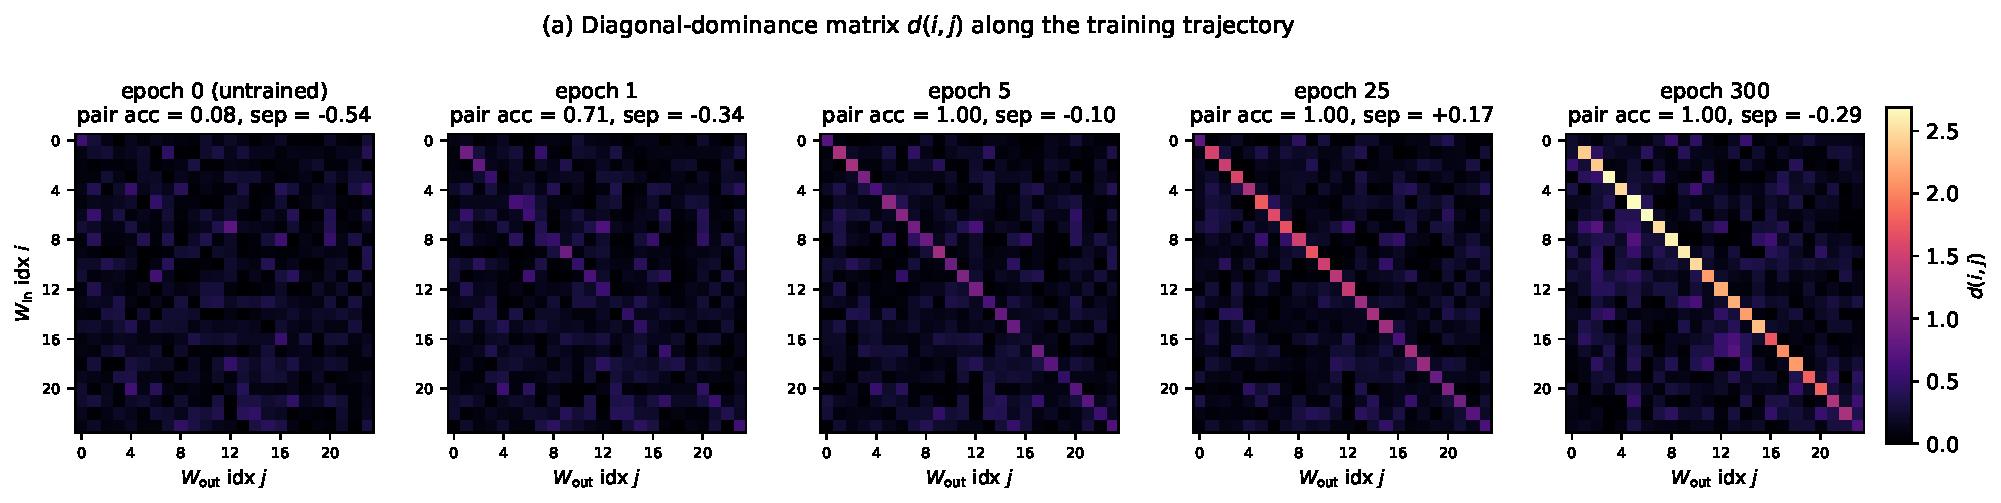
\includegraphics[width=\textwidth]{../figures/fig_null_a_heatmaps.pdf}\\[0.5em]
{\small (a) Training dynamics: 24-block ResNet}\\[1em]
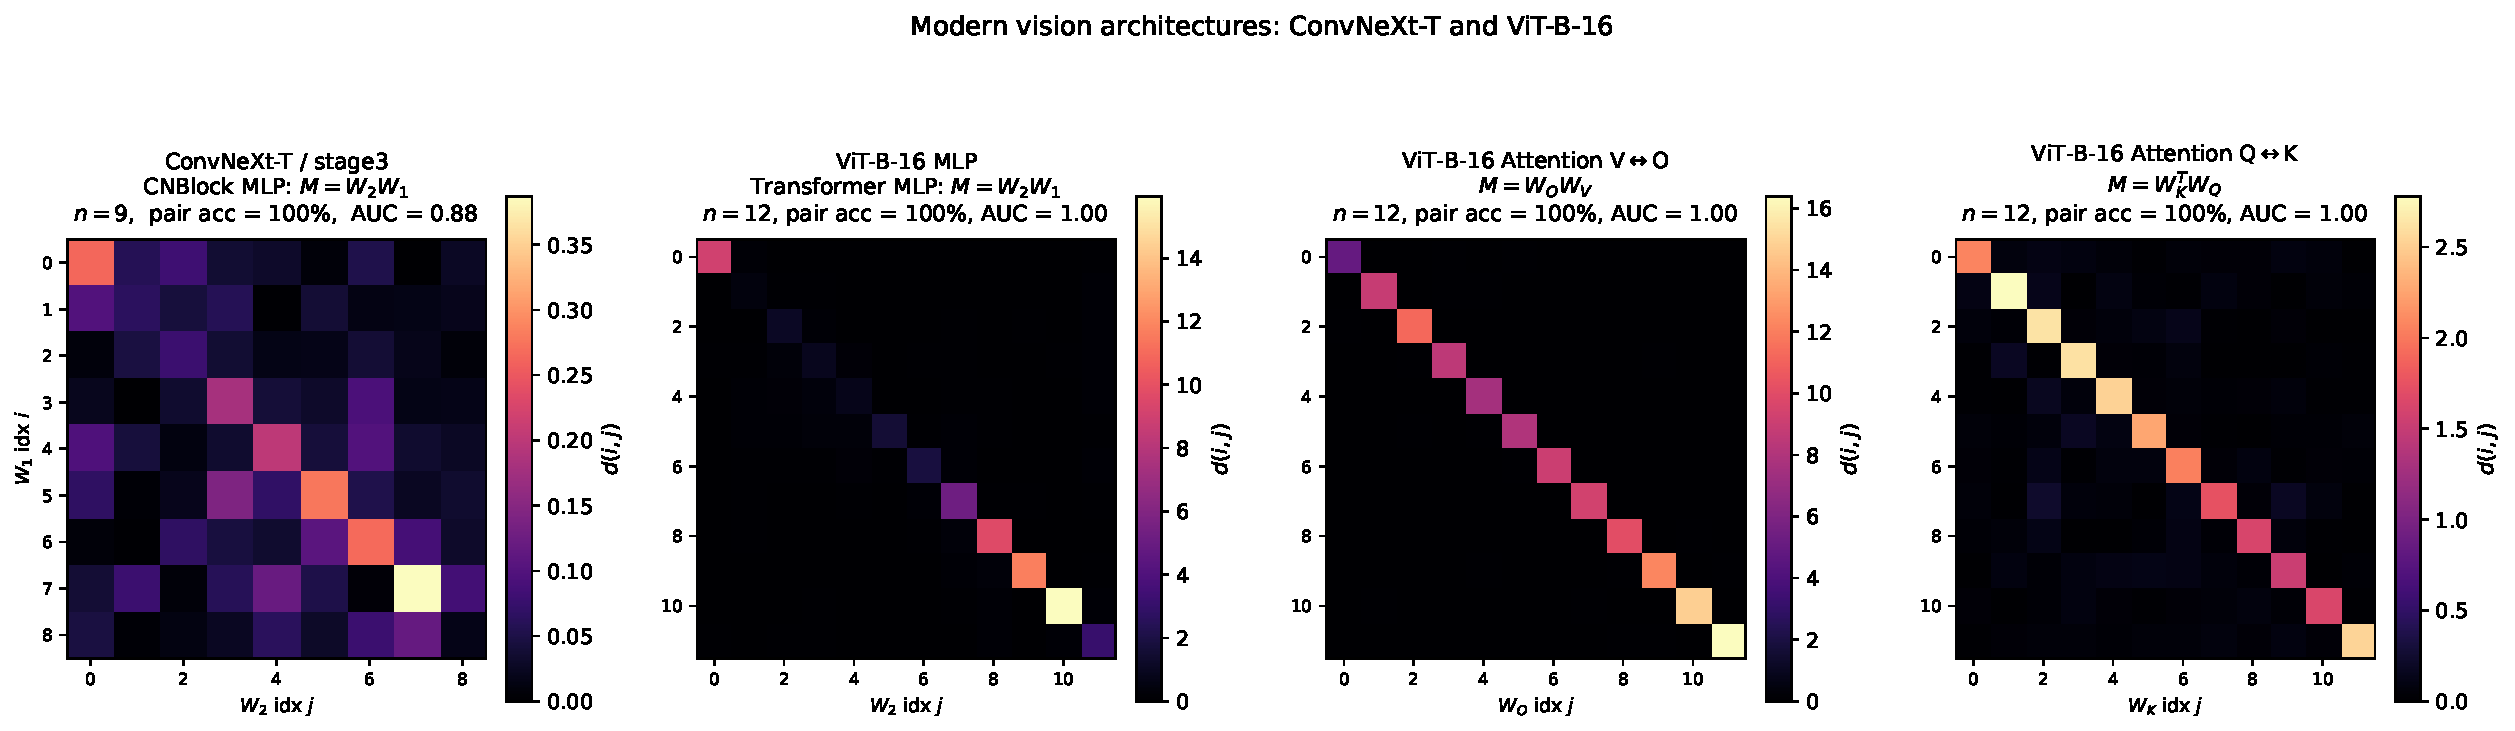
\includegraphics[width=\textwidth]{../figures/fig_modern_vision_pairing.pdf}\\[0.5em]
{\small (b) Modern vision architectures: ViT-B/16 and ConvNeXt-T}
\caption{Diagonal-dominance matrices $d(i,j)$ reveal training-induced structure. \textbf{(a)} At initialization (epoch 0), no diagonal structure is visible. By epoch 5, the diagonal is fully separated and pair accuracy reaches 100\%. \textbf{(b)} ViT-B/16 (MLP, V/O attention, Q/K attention paths) and ConvNeXt-T all achieve 100\% pairing accuracy with clear diagonal structure.}
\label{fig:heatmaps}
\end{figure}

\section{Introduction}\label{sec:intro}

Establishing the provenance of neural network weights has become critical for intellectual property protection, model auditing, and supply chain verification. The dominant approach---embedding watermarks during training---suffers from two fundamental limitations: it requires foresight (the watermark must be inserted before training concludes) and it lacks robustness (fine-tuning or pruning can remove the signal). Post-hoc verification methods based on Frobenius distance or singular value comparison perform little better than chance on standard benchmarks.

We propose a fundamentally different approach, building on a key observation: training itself leaves an indelible fingerprint. Modern architectures use \emph{residual connections}---shortcuts that allow information to bypass layers---to enable training of very deep networks. For these networks to learn effectively, adjacent layers must allow signals to pass through with minimal distortion. This constraint shapes how weights evolve during training: adjacent weight matrices $W_{\text{out}}$ and $W_{\text{in}}$ learn to partially cancel each other out, so their product $W_{\text{out}} W_{\text{in}}$ concentrates near $-\varepsilon I$ for small $\varepsilon$. In plain terms, the diagonal entries dominate the off-diagonal entries---a pattern we call \emph{diagonal dominance}. Crucially, this structure emerges from training dynamics rather than architectural constraints, as confirmed by our null model experiments on randomly initialized networks.

This fingerprint enables retroactive verification: any model trained with residual connections carries this signal, whether or not provenance verification was anticipated. We formalize a \emph{diagonal-dominance score} quantifying this pattern and show it achieves near-perfect classification across transformer architectures (GPT-2 family) and convolutional networks (ViT, ConvNeXt, ResNets). The signal strengthens with model scale and remains robust under substantial adversarial perturbations.

Unlike watermarking, our method opens new possibilities for auditing deployed models and resolving ownership disputes without requiring cooperation from the original trainer. Section~\ref{sec:background} reviews related work, Section~\ref{sec:theory} develops our theoretical framework, Sections~\ref{sec:method}--\ref{sec:experiments} present methodology and evaluation, and Section~\ref{sec:conclusion} discusses implications.

\section{Background and Related Work}\label{sec:background}

\subsection{Watermarking and Ownership Verification}

Verifying ownership of neural network weights has become critical as models represent significant intellectual property. Existing approaches fall into three families, each embedding information during or after training.

\textbf{Embedding-based watermarks} modify the training loss to encode a signature directly into the weights. \citet{uchida2017embedding} pioneered this approach by adding a regularization term that projects a binary string into a subset of convolutional filters. DeepSigns~\citep{rouhani2019deepsigns} extended this to activation maps, while DeepMarks~\citep{chen2019deepmarks} embedded fingerprints that survive model compression.

\textbf{Backdoor-based watermarks} train the network to produce specific outputs on a secret trigger set. \citet{adi2018turning} demonstrated that a model can memorize arbitrary input-output pairs without degrading accuracy on the primary task. \citet{zhang2018protecting} showed similar results across architectures, treating the trigger set as a cryptographic key.

\textbf{Decision-boundary fingerprinting} identifies ownership through carefully crafted inputs near the classification boundary. \citet{le2020adversarial} used adversarial examples as fingerprints, while IPGuard~\citep{cao2021ipguard} selected inputs maximally sensitive to boundary perturbations. These methods require no training modification but depend on preserving the exact decision surface.

A critical limitation unifies all three families: they can be removed or bypassed. \citet{lukas2022sok} systematically evaluated watermarking schemes on image classification and found that fine-tuning, pruning, or model extraction significantly degrades or removes watermarks across all tested methods within realistic compute budgets. This motivates our structurally different approach: rather than embedding information, we read a fingerprint that training itself induces.

\textbf{Comparison with broader model-attribution attacks.} Related lines of work in adversarial machine learning serve adjacent goals but address fundamentally different questions. \emph{Membership inference attacks}~\citep{shokri2017membership} ask whether a particular training example was used to train a model, given black-box query access; they target dataset provenance, not weight provenance. \emph{Model-extraction / knockoff attacks}~\citep{tramer2016stealing, orekondy2019knockoff} reconstruct a functional copy of a target model from query-response pairs, but the resulting student has fresh randomly-initialized weights that bear no structural relation to the teacher. Distillation defenses similarly do not preserve weight-level identity. Our setting is orthogonal: we assume white-box weight access (Section~\ref{sec:background}, threat model) and verify weight-level identity by reading the structural signature that training itself imprints on the residual-branch products. The diagonal-dominance fingerprint therefore complements query-based attribution---it provides the white-box verification step that membership inference and model extraction leave open.

\textbf{Threat model.} We assume white-box verification: the verifier has full access to the model weights. The adversary may fine-tune, prune, permute weight indices, or add noise to the weights, but cannot fundamentally alter the residual architecture without retraining from scratch. This setting matches scenarios where a model is suspected to be stolen and the original owner seeks to prove provenance.

\subsection{Dynamical Isometry and Residual Networks}

Deep networks suffer from vanishing and exploding gradients when layer Jacobians deviate significantly from orthogonality. \citet{saxe2014exact} provided exact solutions for deep linear networks, showing that orthogonal initialization enables efficient learning by preserving gradient norms. \citet{pennington2017isometry} formalized this as \emph{dynamical isometry}: the condition that all singular values of the input-output Jacobian concentrate near unity throughout training.

Residual networks~\citep{he2016deep} achieve dynamical isometry through skip connections. \citet{tarnowski2019dynamical} proved that ResNets satisfy dynamical isometry at initialization when residual branches are scaled appropriately. \citet{zaeemzadeh2020norm} further showed that skip connections preserve gradient norms across depth, explaining why ResNets train stably even with hundreds of layers.

Batch normalization reinforces this structure. \citet{santurkar2018does} demonstrated that BatchNorm smooths the loss landscape rather than reducing internal covariate shift. More relevant to our work, \citet{de2020batch} showed that BatchNorm biases residual blocks toward identity mappings, ensuring that the learned transformation $F(x)$ in each block $x + F(x)$ remains small in norm.

These results have a direct implication for weight structure: when residual blocks maintain near-identity behavior, the product of input and output weight matrices within each block exhibits strong diagonal dominance. We formalize this connection and derive the precise relationship in Section~\ref{sec:theory}.

\textbf{From trainability to verification.} The architectural constraints that enable stable training---skip connections enforcing near-identity residual mappings---simultaneously create a verification opportunity. These constraints impose predictable structure on weight matrices that is difficult to remove without destroying the model's function. Our method exploits this structure as an intrinsic fingerprint.

\subsection{Intrinsic Fingerprinting and Model Attribution}

Recent work has explored fingerprints that emerge from training without explicit embedding. \citet{zheng2022fingerprinting} and \citet{zhao2020shaping} observed that weight statistics can identify models. However, these methods rely on aggregate statistical properties---means, variances, or histogram features of individual weight matrices---which lack the verification precision needed for ownership claims and can be disrupted by simple transformations.

DeepIPR~\citep{fan2019rethinking} introduced passport layers that gate activations, achieving stronger verification but requiring architectural modification. \citet{szyller2021dawn} proposed DAWN for fingerprinting machine-learning-as-a-service APIs, though this targets black-box settings distinct from weight-level verification.

Our approach requires no modification to architecture, loss function, or training procedure. The diagonal-dominance score emerges as a byproduct of dynamical isometry: correctly paired weight matrices from the same residual block exhibit high diagonal dominance in their product, while incorrect pairings score near zero. Crucially, diagonal dominance captures \emph{relational} structure between paired matrices---how they jointly encode the near-identity mapping---rather than aggregate properties of individual matrices. This relational signature is preserved under fine-tuning and noise addition because it reflects the functional constraint that the residual block must approximate, providing robustness against the attacks that defeat embedded watermarks and statistical fingerprints.

\section{Theory}\label{sec:theory}

\subsection{The Diagonal-Dominance Fingerprint}\label{sec:dd-score}

Given input projection $W_{\mathrm{in}}^{(i)} \in \mathbb{R}^{h \times d}$ and output projection $W_{\mathrm{out}}^{(j)} \in \mathbb{R}^{d \times h}$, the diagonal-dominance score is
\begin{equation}\label{eq:dd-score}
  d(i,j) \;=\; \frac{|\mathrm{tr}(W_{\mathrm{out}}^{(j)} W_{\mathrm{in}}^{(i)})|}{\|W_{\mathrm{out}}^{(j)} W_{\mathrm{in}}^{(i)}\|_F}.
\end{equation}
The numerator is the absolute trace of the $d \times d$ product matrix $M := W_{\mathrm{out}}^{(j)} W_{\mathrm{in}}^{(i)}$; the denominator is its Frobenius norm. The ratio measures what fraction of the matrix's total energy concentrates on the diagonal.

Why a ratio rather than the raw trace or Frobenius norm? The trace $|\mathrm{tr}(M)|$ scales with both the intrinsic diagonal structure and the overall magnitude of the weight matrices, which varies across blocks for reasons unrelated to pairing. The Frobenius norm $\|M\|_F$ similarly conflates scale with structure. Their ratio normalizes away scale and isolates the structural signature: a matrix with energy uniformly spread has $d(i,j) = O(1/\sqrt{d})$, while a matrix proportional to the identity achieves the maximum $d(i,j) = \sqrt{d}$. This $\sqrt{d}$ dynamic range is what makes correct pairs distinguishable from incorrect ones.

\subsection{Margin Analysis}\label{sec:margin-analysis}

\paragraph{Motivation.} Given the diagonal-dominance score, the key question is: how well does it separate correct pairs from incorrect ones? We formalize this via a margin analysis.

\paragraph{The trained decomposition.} Dynamic isometry \citep{pennington2017isometry} predicts that a well-trained residual block has Jacobian $J = I + W_{\mathrm{out}} W_{\mathrm{in}}$ close to orthogonal. For the block to act as a near-identity perturbation of the residual stream, the product $W_{\mathrm{out}} W_{\mathrm{in}}$ must approximate a negative scalar multiple of identity. This motivates the decomposition: for a correctly paired block, write
\begin{equation}\label{eq:decomp}
  M := W_{\mathrm{out}}^{(i)} W_{\mathrm{in}}^{(i)} = -\varepsilon I + E,
\end{equation}
where $\varepsilon := |\mathrm{tr}(M)|/d > 0$ captures the diagonal strength and $E$ is the residual with $\mathrm{tr}(E) = 0$. The matrix $E$ contains all off-diagonal structure plus the zero-trace portion of the diagonal. Dynamic isometry implies $\|E\|_F \ll \varepsilon\sqrt{d}$ for well-trained blocks; the following proposition quantifies the margin exactly.

\begin{proposition}[Margin Formula]\label{prop:margin}
Let $M = -\varepsilon I + E$ with $\varepsilon = |\mathrm{tr}(M)|/d$ and $\mathrm{tr}(E) = 0$. Then the diagonal-dominance score satisfies
\begin{equation}\label{eq:margin-formula}
  d(i,i) \;=\; \frac{\sqrt{d}}{\sqrt{1 + \|E\|_F^2 / (\varepsilon^2 d)}} \;\leq\; \sqrt{d},
\end{equation}
with equality if and only if $E = 0$, i.e., $M = -\varepsilon I$.
\end{proposition}

\begin{proof}
By construction, $|\mathrm{tr}(M)| = \varepsilon d$. For the Frobenius norm, expand
\begin{align*}
  \|M\|_F^2 &= \|-\varepsilon I + E\|_F^2 = \varepsilon^2 \|I\|_F^2 - 2\varepsilon \langle I, E \rangle + \|E\|_F^2 \\
            &= \varepsilon^2 d - 2\varepsilon \,\mathrm{tr}(E) + \|E\|_F^2 = \varepsilon^2 d + \|E\|_F^2,
\end{align*}
where the last step uses $\mathrm{tr}(E) = 0$. Substituting into \eqref{eq:dd-score}:
\[
  d(i,i) = \frac{\varepsilon d}{\sqrt{\varepsilon^2 d + \|E\|_F^2}} = \frac{\sqrt{d}}{\sqrt{1 + \|E\|_F^2/(\varepsilon^2 d)}}.
\]
The bound $d(i,i) \leq \sqrt{d}$ follows immediately, with equality iff $\|E\|_F = 0$.
\end{proof}

The margin formula reveals the geometry of diagonal dominance. The numerator $\sqrt{d}$ is the score achievable by a perfect negative-scalar identity; the denominator penalizes deviation from this ideal via the dimensionless ratio $\|E\|_F^2/(\varepsilon^2 d)$. For typical trained blocks in \citet{park2026}'s puzzle network, $\|E\|_F/(\varepsilon\sqrt{d}) \in [1.9, 3.8]$, yielding $d(i,i) \in [1.76, 3.23]$---well above the baseline but below the theoretical maximum of $\sqrt{48} \approx 6.93$. Figure~\ref{fig:margin} verifies that the formula reproduces empirical scores to floating-point precision.

\begin{figure}[H]
\centering
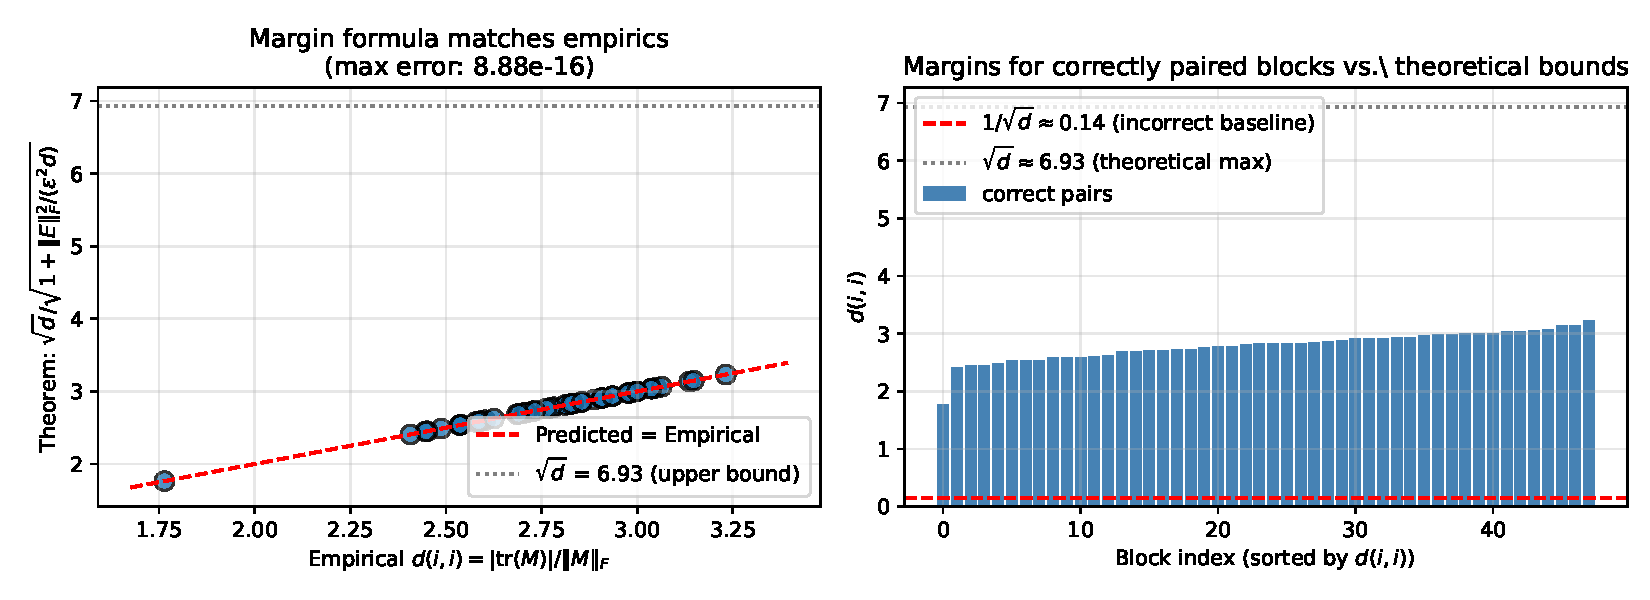
\includegraphics[width=\textwidth]{../figures/fig_margin_theorem.pdf}
\caption{Proposition~\ref{prop:margin} verification. \textbf{Left:} Predicted $d(i,i)$ from the margin formula vs.\ empirical values for all 48 blocks---points lie on the identity line. \textbf{Right:} Sorted correct-pair margins (blue) vs.\ incorrect-pair baseline (red dashed) and theoretical upper bound $\sqrt{d}$ (grey dotted).}
\label{fig:margin}
\end{figure}

\begin{corollary}[Signal-to-Baseline Ratio]\label{cor:baseline}
Suppose $(W_{\mathrm{in}}^{(i)}, W_{\mathrm{out}}^{(j)})$ with $i \neq j$ are independent random matrices with i.i.d.\ zero-mean entries. Then
\begin{equation}\label{eq:baseline}
  \mathbb{E}[d(i,j)^2] = \frac{1}{d}.
\end{equation}
Consequently, the expected score for incorrect pairs is $\mathbb{E}[d(i,j)] \approx 1/\sqrt{d}$, while correct pairs score $d(i,i) = O(\sqrt{d})$ by Proposition~\ref{prop:margin}. The signal-to-baseline ratio scales as $d$.
\end{corollary}

The corollary explains why diagonal-dominance pairing succeeds: correct pairs achieve scores of order $\sqrt{d}$ (diminished from the maximum only by off-diagonal energy $\|E\|_F$), while incorrect pairs score at the random baseline $1/\sqrt{d}$. The gap grows with dimension, providing increasingly robust separation for deeper or wider networks.

\paragraph{The signal requires training.} A skeptical reader might wonder whether diagonal dominance is an artifact of matrix shapes or the residual architecture itself, rather than a learned property. We rule this out with a null model.

\begin{corollary}[Null Model]\label{cor:null-model}
For randomly initialized weights with no training, all pairs---correct and incorrect---satisfy
\begin{equation}\label{eq:null}
  \mathbb{E}[d(i,j)] = \frac{1}{\sqrt{d}} + o(1)
\end{equation}
uniformly in $(i,j)$. Hungarian matching on $-d$ recovers correct pairs at the chance rate $1/D$.
\end{corollary}

This follows immediately from Corollary~\ref{cor:baseline}: without training, there is no mechanism coupling $W_{\mathrm{in}}^{(i)}$ with $W_{\mathrm{out}}^{(i)}$ more than with any other $W_{\mathrm{out}}^{(j)}$. The decomposition \eqref{eq:decomp} does not hold because $\varepsilon$ is not systematically positive for $i = j$.

\paragraph{Empirical verification.} We instantiate the null model on a network matching \citet{park2026}'s architecture (depth 48, hidden dimension 96, input/output dimension 48), with Kaiming initialization and no training. Pair accuracy is $6.25\%$ (chance is $1/48 \approx 2.08\%$; the small excess is Hungarian's bias toward the optimum). Pair separation---the gap between the worst correct-pair score and the best incorrect-pair score---is $-0.42$. On the trained puzzle network, these metrics become: pair accuracy $100\%$, pair separation $+1.18$, and a $21\times$ ratio between correct-pair and incorrect-pair means. The transformation occurs within the first few epochs of training (Figure~\ref{fig:heatmaps}).

\paragraph{What this rules out.} The null model eliminates three alternative explanations: (a)~diagonal dominance is not an artifact of compatible matrix shapes; (b)~the residual connection itself does not create the signal; (c)~any nontrivial loss level does not suffice. The diagonal-dominance fingerprint is a \emph{learned} property induced by gradient descent, exactly as dynamical isometry theory predicts.

\section{Methodology}\label{sec:method}

This section describes the practical procedure for recovering layer pairings from weight matrices. The theoretical justification appears in Section~\ref{sec:theory}; here we specify \emph{what} to compute and \emph{how}.

\subsection{Diagonal-Dominance Pairing}\label{sec:pairing}

Given $L$ input projections $\{W_{\mathrm{in}}^{(i)}\}_{i=1}^L$ and $L$ output projections $\{W_{\mathrm{out}}^{(j)}\}_{j=1}^L$ with unknown correspondence, we recover the pairing as follows.

\paragraph{Step 1: Score matrix.} For each pair $(i,j) \in [L] \times [L]$, compute the diagonal-dominance score $d(i,j)$ via \eqref{eq:dd-score}, yielding an $L \times L$ matrix $D$. By Proposition~\ref{prop:margin}, correctly paired blocks satisfy $d(i,i) = O(\sqrt{d})$ while incorrect pairs have $\mathbb{E}[d(i,j)] = O(1/\sqrt{d})$.

\paragraph{Step 2: Hungarian matching.} Run the Hungarian algorithm on the cost matrix $-D$ (negated because Hungarian minimizes). The output is a permutation $\hat\pi$ assigning input $i$ to output $\hat\pi(i)$. Ground truth is the identity permutation.

\paragraph{Complexity.} Computing $D$ requires $L^2$ matrix products, each $O(dh)$ for hidden dimension $h$. Hungarian matching runs in $O(L^3)$. For $L{=}48$, $d{=}48$, $h{=}96$, the full procedure executes in under one second on CPU.

\paragraph{Architecture-aware factorization.} The procedure above assumes a two-factor residual branch $x + W_{\mathrm{out}} \phi(W_{\mathrm{in}} x)$. For architectures with deeper residual branches, the diagonal-dominance score must be computed on the \emph{complete} branch product. Table~\ref{tab:factorization} summarizes the correct factorization for each architecture family we evaluate.

\begin{table}[t]
\centering
\small
\begin{tabular}{lll}
\toprule
Architecture & Residual branch & Branch product $M$ \\
\midrule
Residual MLP / BasicBlock & $x + W_2 \phi(W_1 x)$ & $W_2 W_1$ \\
Transformer MLP & $x + W_2 \phi(W_1 \mathrm{LN}(x))$ & $W_2 W_1$ \\
Attention V/O path & $x + W_O \mathrm{Attn}(W_V x)$ & $W_O W_V$ \\
Attention Q/K path & $\mathrm{softmax}(Q K^\top / \sqrt{d})$ & $W_Q W_K^\top$ \\
Bottleneck ResNet & $x + W_3 \phi(W_2 \phi(W_1 x))$ & $W_3 W_2 W_1$ \\
ConvNeXt MLP & $x + W_2 \phi(W_1 \mathrm{LN}(x))$ & $W_2 W_1$ \\
\bottomrule
\end{tabular}
\caption{Architecture-aware factorization. The diagonal-dominance score is computed on the complete residual-branch product. Two-factor branches (MLPs, BasicBlocks, attention paths) use $M = W_{\mathrm{out}} W_{\mathrm{in}}$; three-factor branches (Bottleneck ResNets) require the full triple product $M = W_3 W_2 W_1$. The naive endpoint product $W_3 W_1$ fails for Bottleneck blocks because it skips the middle convolution that performs feature mixing.}
\label{tab:factorization}
\end{table}

\subsection{Weight Extraction for Modern Architectures}\label{sec:architectures}

We describe how to extract the appropriate weight products from each architecture family.

\paragraph{Transformer MLPs.} Transformer MLP sublayers have the residual form $\mathrm{MLP}(x) = x + W_2 \cdot \mathrm{GELU}(W_1 \cdot \mathrm{LN}(x))$, where $W_1 \in \mathbb{R}^{4d \times d}$ expands and $W_2 \in \mathbb{R}^{d \times 4d}$ contracts. The product $W_2 W_1 \in \mathbb{R}^{d \times d}$ plays the role of $W_{\mathrm{out}} W_{\mathrm{in}}$, so the pairing procedure applies directly. For GPT-2, we extract \texttt{c\_fc} ($W_1$) and \texttt{c\_proj} ($W_2$) from each transformer block.

\paragraph{Transformer attention.} Attention sublayers admit two distinct pairing paths:
\begin{itemize}[leftmargin=*,itemsep=2pt]
  \item \textbf{V/O path (residual write):} The value-to-output projection $M = W_O W_V \in \mathbb{R}^{d \times d}$ captures how attention writes to the residual stream.
  \item \textbf{Q/K path (attention-score coupling):} The query-key interaction $M = W_Q W_K^\top \in \mathbb{R}^{d \times d}$ determines which positions attend to which.
\end{itemize}

\paragraph{Vision Transformers (ViT).} ViT encoder blocks contain standard MLP and multi-head attention sublayers. The MLP path uses $W_2 W_1$ identically to GPT-2. For attention, we reshape the per-head projections into block-diagonal matrices and compute the full V/O and Q/K products.

\paragraph{Convolutional networks with BatchNorm.} For ImageNet ResNets, we apply two preprocessing steps before computing the branch product:
\begin{enumerate}[leftmargin=*,itemsep=2pt]
  \item \textbf{Spatial collapse:} Convolutional kernels are projected to channel-mixing matrices by either summing over spatial positions (\emph{channel-sum}) or extracting the center tap (\emph{center-tap}).
  \item \textbf{BatchNorm folding:} The BatchNorm affine transformation $\gamma / \sqrt{\sigma^2 + \epsilon}$ is folded into the adjacent convolution's output channels.
\end{enumerate}
For \textbf{BasicBlock} architectures (ResNet-18, ResNet-34), the two-factor product $M = W_2 W_1$ applies. For \textbf{Bottleneck} architectures (ResNet-50, ResNet-101, ResNet-152), the three-factor product $M = W_3 W_2 W_1$ is required---the naive endpoint product $W_3 W_1$ skips the $3 \times 3$ middle convolution that performs spatial feature mixing.

\paragraph{ConvNeXt.} ConvNeXt blocks use depthwise separable convolutions followed by a Linear$\to$GELU$\to$Linear MLP. The depthwise convolution operates per-channel and does not mix channels; channel mixing occurs exclusively in the MLP path, so the branch product is $M = W_2 W_1$.

\subsection{Verification Protocol}\label{sec:verification}

For forensic applications---confirming a deployed model matches a registered checkpoint or detecting unauthorized derivatives---the procedure is:

\begin{enumerate}[leftmargin=*,itemsep=2pt]
  \item \textbf{Register.} At deployment, store the weight matrices $\{W_{\mathrm{in}}^{(k)}, W_{\mathrm{out}}^{(k)}\}_{k=1}^L$ and their canonical ordering.
  \item \textbf{Extract.} From the suspect model, extract the corresponding weights (potentially reordered or fine-tuned).
  \item \textbf{Pair.} Run diagonal-dominance Hungarian matching on the suspect weights to recover $\hat\pi$.
  \item \textbf{Compare.} Measure pair accuracy: $|\{i : \hat\pi(i) = i\}|/L$. Perfect recovery indicates the suspect derives from the registered checkpoint.
\end{enumerate}

\section{Experiments}\label{sec:experiments}

We organize our experiments around five research questions that systematically validate the diagonal-dominance fingerprint: core validation across architectures (RQ1), scalability to large models (RQ2), comparison to alternative methods (RQ3), robustness to post-training modifications (RQ4), and mechanistic understanding of the signal's origin (RQ5).

\subsection{RQ1: Core Method Validation}

The central methodological question is whether the diagonal-dominance signature reliably recovers layer ordering across different neural network architectures. We validate this across five architecture families: residual MLPs, Transformers (GPT-2 and ViT), ImageNet ResNets with BatchNorm, modern ConvNets, and a cross-family transformer sweep (BERT, Mistral-7B).

\paragraph{Transformers.}
On pretrained GPT-2 models spanning 124M to 1.5B parameters (12--48 layers), diagonal-dominance Hungarian matching achieves \textbf{100\% pairing accuracy} on MLP blocks across all four model sizes. The signal strength increases with model scale: mean correct-pair score rises from $4.18$ (GPT-2) to $7.77$ (GPT-2-xl). Between 81--92\% of correctly paired products exhibit negative traces, consistent with dynamic isometry. A randomly initialized GPT-2 baseline achieves only 17\% accuracy (chance is 8.3\%), confirming the signal is training-induced.

For attention paths, we evaluate both the value-output coupling ($W_O W_V$) and query-key coupling ($W_Q W_K^\top$). On GPT-2-xl, both paths achieve \textbf{100\% accuracy} (Figure~\ref{fig:attention}). On ViT-B/16, the $V\!\leftrightarrow\!O$ path produces the strongest signal in our study: pair separation of \textbf{+4.84}, AUC of \textbf{1.000}, and 100\% of correctly paired products showing negative trace---the full theoretical prediction. The $Q\!\leftrightarrow\!K$ path also recovers \textbf{100\%} with separation +1.42.

\begin{figure}[H]
\centering
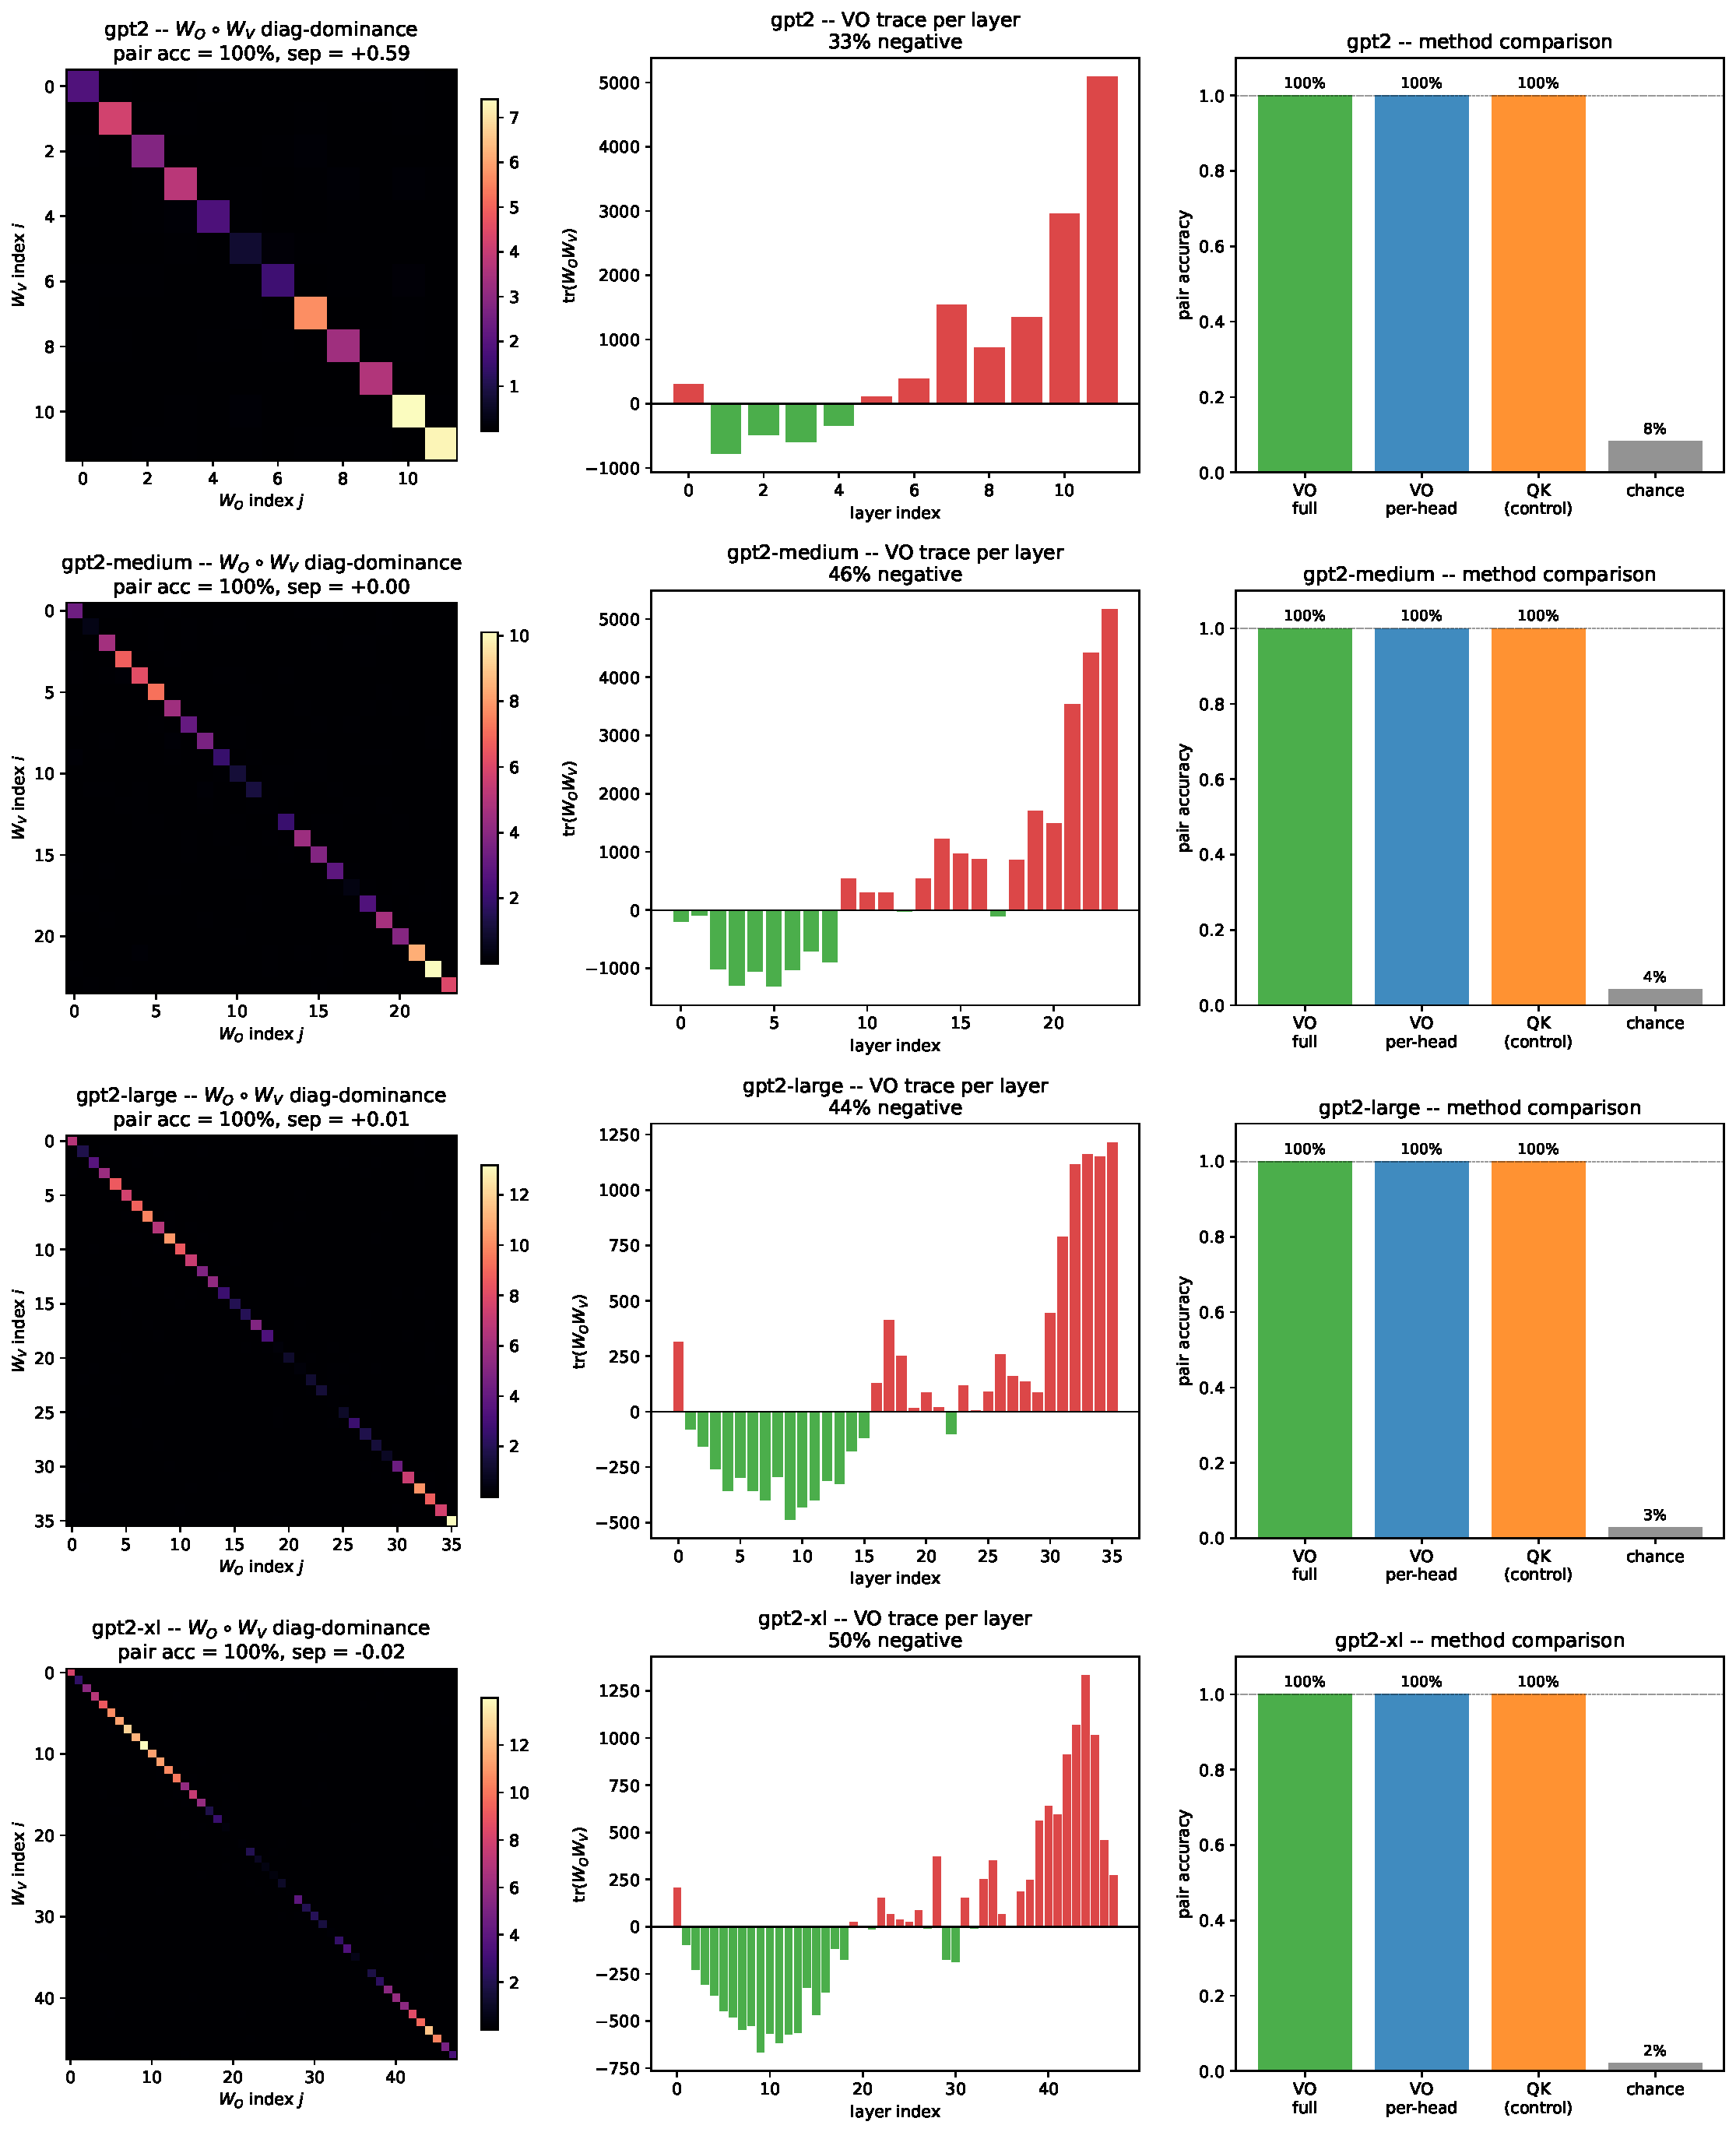
\includegraphics[width=\textwidth]{../figures/fig_gpt2_attention_pairing.pdf}
\caption{Attention path pairing results. Diagonal-dominance matrices for the V/O path (value-to-output projection) and Q/K path (query-key coupling) across GPT-2 model sizes. Both paths achieve 100\% pairing accuracy.}
\label{fig:attention}
\end{figure}

\paragraph{ImageNet ResNets with BatchNorm.}
For ResNet Bottleneck blocks (ResNet-50 through ResNet-152), the naive endpoint product $W_3 W_1$ fails completely, achieving only chance-level accuracy. However, using the architecture-aware \emph{triple} product $W_3 W_2 W_1$ restores recovery to \textbf{91--100\%} across stages up to 35 blocks. Specifically: ResNet-50/layer3 ($n{=}5$) achieves 100\% with AUC 1.000; ResNet-101/layer3 ($n{=}22$) achieves 100\% with AUC 0.995; ResNet-152/layer3 ($n{=}35$) achieves 91\% with AUC 0.964. Random-init baselines remain at chance, confirming the signal is training-induced even under BatchNorm. Figure~\ref{fig:resnet_factorization} illustrates the critical difference between wrong and correct factorization.

\begin{figure}[H]
\centering

\includegraphics[width=\textwidth]{../figures/fig_resnet_wrong_vs_correct_factorization.pdf}
\caption{Architecture-aware factorization for Bottleneck ResNets. \textbf{Left:} The naive endpoint product $W_3 W_1$ shows no diagonal structure. \textbf{Right:} The correct triple product $W_3 W_2 W_1$ reveals clear diagonal dominance, enabling perfect pairing.}
\label{fig:resnet_factorization}
\end{figure}

\paragraph{Modern Vision Architectures.}
ConvNeXt-T stage~3 (9 CNBlocks with LayerNorm) achieves \textbf{100\%} pairing accuracy via the MLP product $W_2 W_1$, with AUC 0.875. Random-init baselines over 20 seeds show $8.3\%\pm 8.0\%$ accuracy (chance 11.1\%). ViT-B/16 achieves \textbf{100\%} on all three paths---MLP, attention V/O, and attention Q/K---each with AUC 1.000. Figure~\ref{fig:heatmaps}(b) shows results across these modern vision architectures.

\paragraph{Cross-family transformer generality.}
To test whether the fingerprint is specific to GPT-style causal decoders with GELU MLPs, we evaluate three further families: encoder-only \emph{BERT-base} \citep{devlin2019bert} (12 layers, bidirectional self-attention, MLM-pretrained, GELU); the SwiGLU+GQA decoder-only \emph{Mistral-7B} \citep{jiang2023mistral7b} (32 layers, sliding-window attention, grouped-query attention with $n_{\text{kv}}{=}8$); and \emph{LLaMA-2-7B} \citep{touvron2023llama2} in both base and RLHF-tuned chat variants (32 layers, SwiGLU, RMSNorm, full multi-head attention with $n_{\text{kv}}{=}32$). For SwiGLU MLPs we score three architecture-aware factorizations---$W_{\text{down}}W_{\text{up}}$, $W_{\text{down}}W_{\text{gate}}$, and the joint stack $W_{\text{down}}[W_{\text{up}};W_{\text{gate}}]$---and expand the GQA $W_K,W_V$ projections from 8 heads to 32 before scoring on Mistral. All four families recover \textbf{100\%} of correct pairs on \emph{every} path (Table~\ref{tab:transformer_family}); random-init baselines collapse to $\le\!6\%$ (BERT) and $\le\!9\%$ (Mistral, LLaMA-2). This rules out three potential confounds at once: the signal is not specific to GELU activations (SwiGLU works), not specific to causal masking (bidirectional and sliding-window both work), and not specific to full attention (8-way GQA still gives AUC 1.000 on $W_OW_V$). The base$\to$chat comparison on LLaMA-2 is a direct robustness probe: RLHF fine-tuning preserves the fingerprint exactly on every path, with pair separations matching the base model to within $\pm 0.005$ on four of five paths; only $W_OW_V$ shows a measurable but non-fatal separation drop ($+0.141\to +0.036$), indicating that RLHF perturbs the attention output projection more than the MLP or Q/K paths but does not destroy the diagonal mass. Notably, BERT MLP and the SwiGLU $W_{\text{down}}W_{\text{gate}}$ path exhibit only $8\%$ and $38\%$--$62\%$ negative traces respectively and their pair separations are slightly negative, yet Hungarian assignment still recovers every pair: negative trace is \emph{sufficient} but not necessary for identifiability---the broader fingerprint is concentration of diagonal mass in the correct branch product, which the global assignment optimum is robust enough to exploit even when row-wise dominance is absent.

\begin{table}[h]
\centering
\small
\renewcommand{\arraystretch}{1.05}
\begin{tabular}{llccc}
\toprule
Model & Path & Pair Acc & AUC & Random Acc \\
\midrule
BERT-base       & MLP $W_2 W_1$                          & 100\% & 0.970 & 6\% $\pm$ 5\% \\
BERT-base       & Attn $W_O W_V$                         & 100\% & 1.000 & 3\% $\pm$ 5\% \\
BERT-base       & Attn $W_Q W_K^\top$                    & 100\% & 0.972 & 6\% $\pm$ 5\% \\
\midrule
Mistral-7B      & MLP $W_{\text{down}} W_{\text{up}}$    & 100\% & 1.000 & 2\% $\pm$ 2\% \\
Mistral-7B      & MLP $W_{\text{down}} W_{\text{gate}}$  & 100\% & 0.989 & 2\% $\pm$ 2\% \\
Mistral-7B      & MLP joint stack                        & 100\% & 1.000 & 2\% $\pm$ 2\% \\
Mistral-7B      & Attn $W_O W_V$ (GQA)                   & 100\% & 1.000 & 1\% $\pm$ 2\% \\
Mistral-7B      & Attn $W_Q W_K^\top$ (GQA)              & 100\% & 1.000 & 2\% $\pm$ 4\% \\
\midrule
LLaMA-2-7B      & MLP $W_{\text{down}} W_{\text{up}}$    & 100\% & 1.000 & 6\% \\
LLaMA-2-7B      & MLP $W_{\text{down}} W_{\text{gate}}$  & 100\% & 0.966 & 3\% \\
LLaMA-2-7B      & MLP joint stack                        & 100\% & 1.000 & 9\% \\
LLaMA-2-7B      & Attn $W_O W_V$                         & 100\% & 1.000 & 9\% \\
LLaMA-2-7B      & Attn $W_Q W_K^\top$                    & 100\% & 1.000 & 6\% \\
\midrule
LLaMA-2-7B-chat & MLP $W_{\text{down}} W_{\text{up}}$    & 100\% & 1.000 & 6\% \\
LLaMA-2-7B-chat & MLP $W_{\text{down}} W_{\text{gate}}$  & 100\% & 0.964 & 3\% \\
LLaMA-2-7B-chat & MLP joint stack                        & 100\% & 1.000 & 9\% \\
LLaMA-2-7B-chat & Attn $W_O W_V$                         & 100\% & 1.000 & 9\% \\
LLaMA-2-7B-chat & Attn $W_Q W_K^\top$                    & 100\% & 1.000 & 6\% \\
\bottomrule
\end{tabular}
\caption{Cross-family transformer pairing. The fingerprint generalizes across encoder-only (BERT), SwiGLU+GQA decoder-only (Mistral), and SwiGLU full-MHA decoder-only (LLaMA-2); the base$\to$chat comparison on LLaMA-2 shows RLHF fine-tuning preserves the fingerprint at 100\% pair accuracy across all paths. Random-init baselines for BERT and Mistral are averaged over 3 seeds; LLaMA-2 random rows use 1 seed (laptop compute budget). GQA $W_K,W_V$ expanded from 8 to 32 heads before scoring on Mistral.}
\label{tab:transformer_family}
\end{table}

\subsection{RQ2: Scalability}

How does the method perform as model size increases from millions to billions of parameters? Table~\ref{tab:gpt2_scaling} summarizes the scaling behavior of MLP block pairing across the GPT-2 family.

\begin{table}[t]
\centering
\small
\renewcommand{\arraystretch}{1.1}
\begin{tabular}{lccccc}
\toprule
Model & Params & Layers & Pair Acc & Mean $d(i,i)$ & Neg Traces \\
\midrule
GPT-2        & 124M  & 12 & 100\% & 4.18 & 92\% \\
GPT-2-medium & 355M  & 24 & 100\% & 5.46 & 92\% \\
GPT-2-large  & 774M  & 36 & 100\% & 6.98 & 81\% \\
GPT-2-xl     & 1.5B  & 48 & 100\% & 7.77 & 81\% \\
\midrule
GPT-2 (random init) & 124M & 12 & 17\% & 0.12 & 50\% \\
\bottomrule
\end{tabular}
\caption{Scalability of MLP block pairing across the GPT-2 family. Pair accuracy remains at 100\% from 124M to 1.5B parameters, while signal strength (mean $d(i,i)$) increases with model size, consistent with the $O(\sqrt{d})$ scaling predicted by Corollary~\ref{cor:baseline}.}
\label{tab:gpt2_scaling}
\end{table}

Signal strength \emph{increases} with model size: mean $d(i,i)$ grows from 4.18 (GPT-2, $d{=}768$) to 7.77 (GPT-2-xl, $d{=}1600$). The fraction of correctly paired products exhibiting negative traces (81--92\%) confirms that dynamical isometry holds in transformer MLP blocks. Figure~\ref{fig:gpt2} visualizes the pairing matrices and trace distributions. These results establish that the diagonal-dominance fingerprint not only persists but \emph{strengthens} as models scale to billions of parameters.

\begin{figure}[H]
\centering

\includegraphics[width=\textwidth]{../figures/fig_gpt2_mlp_pairing.pdf}
\caption{GPT-2 MLP pairing results. \textbf{Left:} Diagonal-dominance matrices for GPT-2 (124M, 12 layers) and GPT-2-XL (1.5B, 48 layers)---bright diagonals indicate perfect pairing. \textbf{Center:} Trace values per layer; 81--92\% are negative, consistent with dynamical isometry. \textbf{Right:} Method comparison showing diagonal-dominance achieves 100\% accuracy while Frobenius matching plateaus at 47--67\%.}
\label{fig:gpt2}
\end{figure}

\subsection{RQ3: Comparison to Alternative Methods}

Establishing that diagonal dominance outperforms alternative approaches is essential for validating the method's practical utility. We compare against two natural baselines: Frobenius norm matching and singular-value distance.

Diagonal dominance achieves perfect pairing accuracy (100\%) on all four GPT-2 variants. In contrast, \textbf{Frobenius norm matching degrades substantially with model size}, dropping from 67\% on GPT-2 to 47\% on GPT-2-large. \textbf{Singular-value distance performs at or below chance} (0--8\% versus 2.1--8.3\% random baseline), providing no useful pairing signal.

The right panel of Figure~\ref{fig:gpt2} visualizes this comparison directly. On Park's puzzle network, while Frobenius matching also recovers all 48 correct pairs, its minimum per-row margin is only 0.005 compared to 1.36 for diagonal dominance---a $250\times$ gap. More critically, the global Frobenius separation is \emph{negative}, meaning correct pairs cannot be distinguished from incorrect pairs without Hungarian assignment's global optimization. This fragility explains Frobenius matching's degradation on larger transformers.

The key finding is that diagonal dominance captures relational structure that alternative methods miss. Dividing by $\|M\|_F$ normalizes away scale variation and isolates the trace contribution that only correctly paired products possess.

\subsection{RQ4: Robustness to Post-Training Modifications}

For diagonal-dominance fingerprints to serve as a reliable verification mechanism, the layer ordering signal must survive common post-training modifications. We evaluate robustness across three attack families totaling 21 configurations: (i) same-target fine-tuning at learning rates $\{10^{-5}, 10^{-4}, 10^{-3}\}$ for up to 50 epochs; (ii) alternative-target fine-tuning with varying label drift; and (iii) Gaussian weight noise at 7 levels from 1\% to 20\% relative perturbation.

As shown in Figure~\ref{fig:attack}, the diagonal-dominance signal exhibits remarkable robustness. Across all 21 attack configurations, Hungarian matching achieves \textbf{100\% pair accuracy} ($48/48$ pairs recovered). Pair separation degrades gracefully from $+1.18$ (untouched weights) to approximately $+0.93$ after aggressive fine-tuning, but the signal remains well above the decision boundary.

The signal becomes brittle only at approximately \textbf{20\% relative weight noise}---the threshold at which model accuracy itself collapses. For all attacks tested, any erosion of the fingerprint comes hand-in-hand with proportional model damage. There is no ``free lunch'' for an attacker: evading detection requires either retraining effectively from scratch or accepting catastrophic accuracy loss.

\begin{figure}[H]
\centering
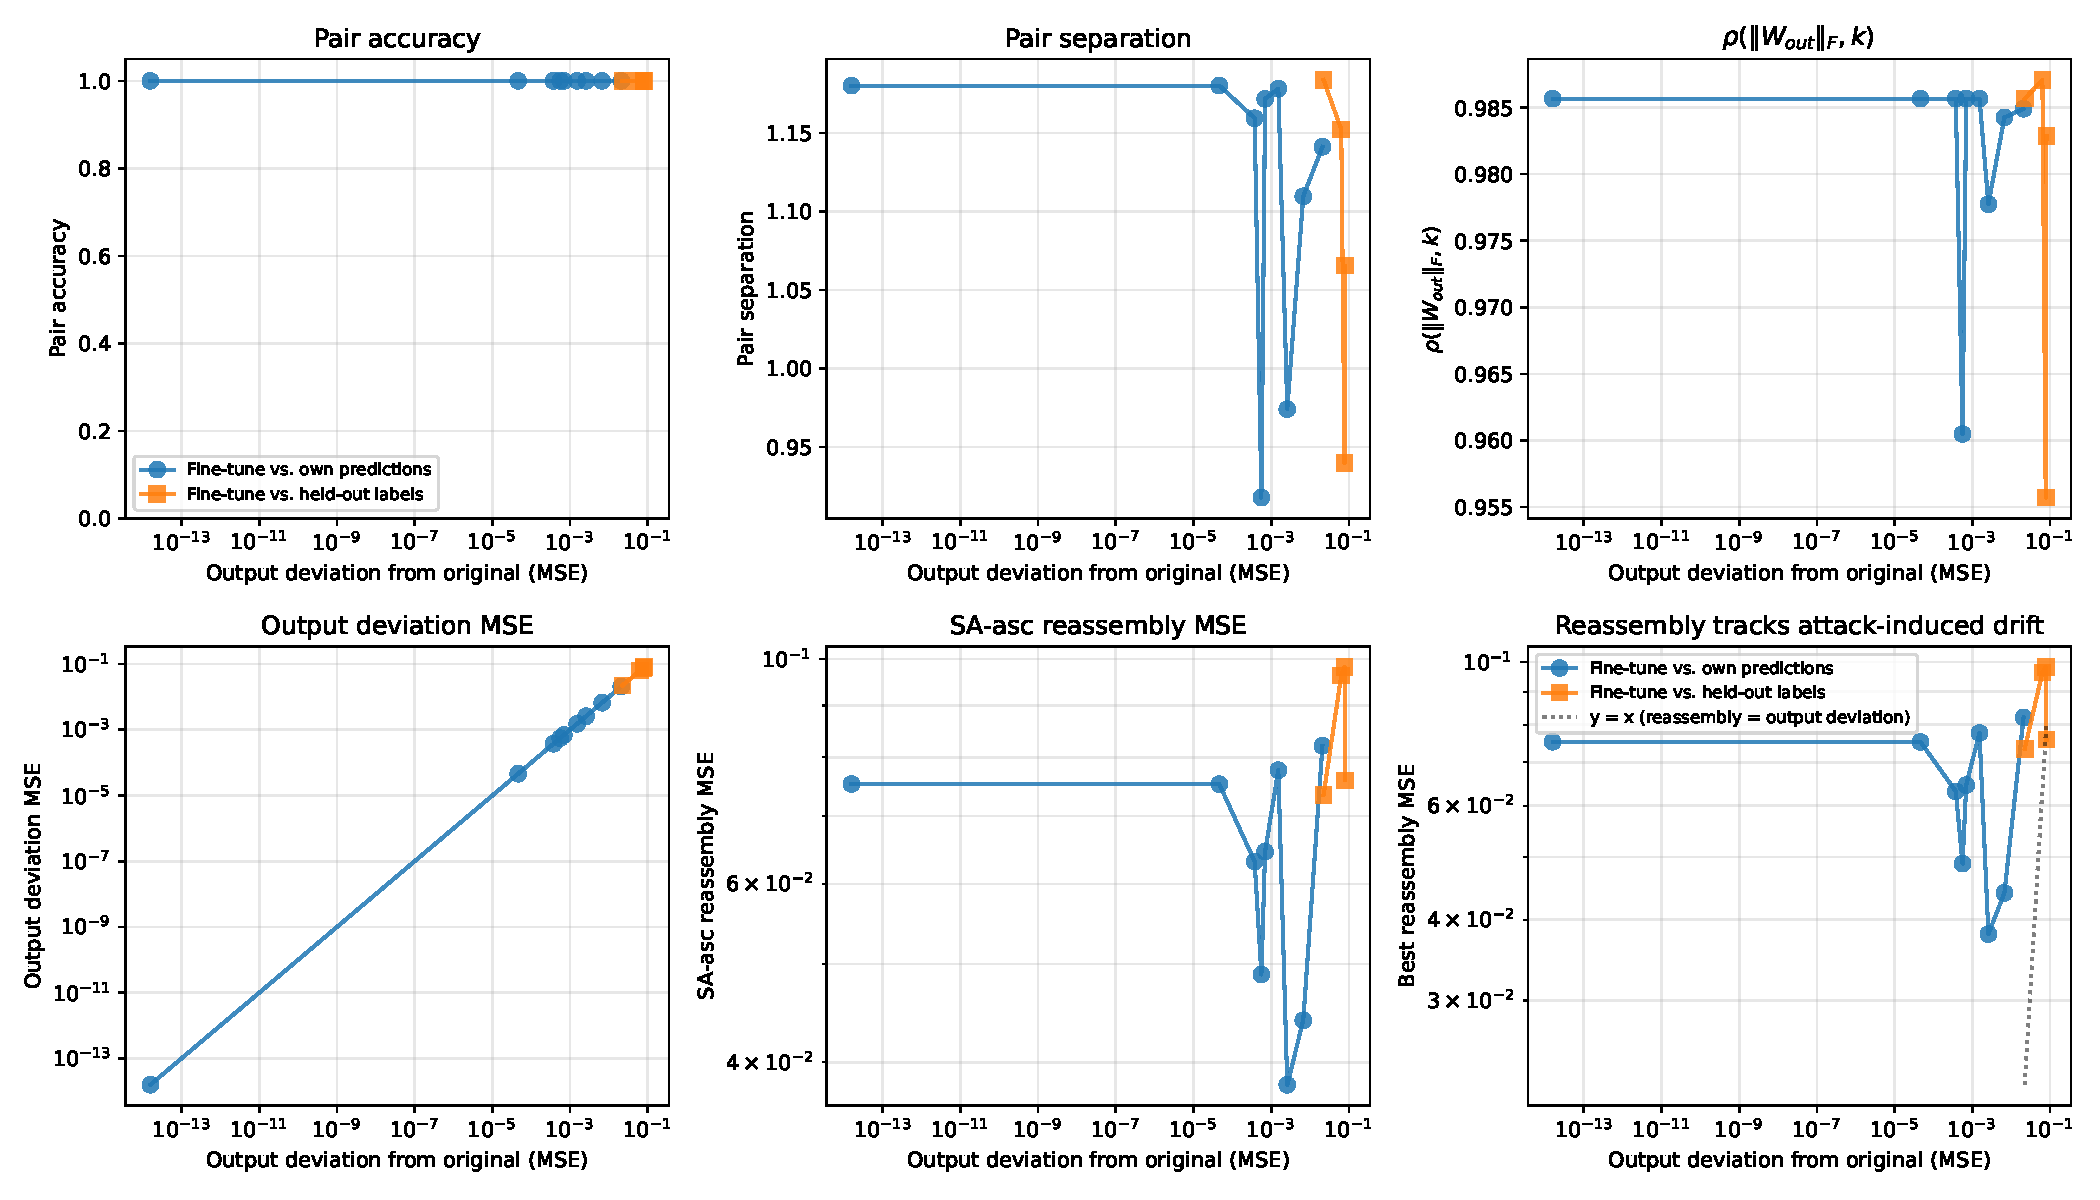
\includegraphics[width=\textwidth]{../figures/fig_attack_robustness.pdf}
\caption{Identifiability under adversarial conditions. \textbf{Left:} Fine-tuning on the original task at various learning rates and epochs. \textbf{Center:} Fine-tuning on alternative targets. \textbf{Right:} Gaussian weight noise. Pair accuracy remains 100\% across all configurations until noise exceeds ${\sim}20\%$ relative magnitude.}
\label{fig:attack}
\end{figure}

\subsection{RQ5: Mechanistic Understanding}

Understanding the \emph{mechanism} behind diagonal dominance establishes whether the signal is a fundamental consequence of residual-block training. We address this through three complementary analyses.

\paragraph{Null model: the signal requires training.}
Corollary~\ref{cor:null-model} predicts that randomly initialized networks should exhibit no diagonal structure. We verify this across seven initialization schemes---Kaiming (uniform and normal), Xavier (uniform and normal), Gaussian, uniform, and orthogonal---on a network with depth 48 and hidden dimension 96. Critically, \emph{orthogonal initialization} is of particular interest: it provides dynamical isometry at initialization by construction, so if the diagonal-dominance signal were an artifact of near-orthogonal Jacobians rather than learned structure, orthogonal init should show elevated pair accuracy even before training. Table~\ref{tab:init_ablation} shows that all seven schemes achieve ${\leq}2.1\%$ pair accuracy at initialization (chance is $2.08\%$), including orthogonal init at exactly $0\%$. After training, all schemes rise to $75$--$100\%$ accuracy. This rules out the hypothesis that the fingerprint is an initialization artifact: even when dynamical isometry is present at initialization, the diagonal-dominance \emph{pairing} signal emerges only through gradient descent.

\begin{table}[h]
\centering
\small
\begin{tabular}{lcc}
\toprule
Initialization & Untrained & Trained \\
\midrule
Kaiming uniform & 2.1\% & 98.6\% \\
Kaiming normal & 2.1\% & 97.2\% \\
Xavier uniform & 2.1\% & 100\% \\
Xavier normal & 2.1\% & 98.6\% \\
Gaussian & 2.1\% & 75.0\% \\
Uniform & 2.1\% & 93.8\% \\
Orthogonal & 0.0\% & 100\% \\
\bottomrule
\end{tabular}
\caption{Initialization scheme ablation. Pair accuracy before and after training across seven initialization schemes. All schemes show chance-level accuracy (${\leq}2.1\%$) at initialization, rising to $75$--$100\%$ after training. Orthogonal initialization---which provides dynamical isometry at init---shows \emph{zero} correct pairs before training, confirming the signal is learned.}
\label{tab:init_ablation}
\end{table}

\paragraph{Training dynamics: emergence by epoch 5.}
Figure~\ref{fig:heatmaps} shows the pairing matrix at five points along the training trajectory. At initialization, no diagonal structure is visible. By epoch 5, the diagonal is fully separated and Hungarian matching recovers $100\%$ of correct pairs. The mean correct-pair score rises monotonically from $0.19$ at epoch 0 to $2.07$ at epoch 300, while the mean incorrect-pair score remains flat at ${\approx}0.16$.

\paragraph{Margin formula verification.}
Proposition~\ref{prop:margin} provides an exact closed-form expression for diagonal dominance. On the 48-block network, this formula reproduces the empirical $d(i,i)$ to floating-point precision on every block (Figure~\ref{fig:margin}). The fitted off-diagonal ratio $\|E\|_F/(\varepsilon\sqrt{d})$ ranges from $1.90$ to $3.80$ across blocks, yielding $d(i,i) \in [1.76, 3.23]$, well below the theoretical maximum of $\sqrt{48} \approx 6.93$ but sufficient for perfect separation.

\paragraph{Initialization ablation: training enforces isometry from non-isometric starts.}
A skeptical reading of dynamical-isometry theory is that the diagonal-dominance fingerprint requires the network to begin training in a near-isometric state---e.g., from explicit orthogonal initialization. To test this, we re-train 24-block residual MLPs from four common initialization schemes (3 seeds each, 200 epochs, identical optimizer): orthogonal (theoretical sweet spot), Kaiming-normal ($\mathcal{N}(0, \sqrt{2/d_{\mathrm{in}}})$), Xavier-normal ($\mathcal{N}(0, \sqrt{2/(d_{\mathrm{in}}{+}d_{\mathrm{out}})})$), and a small-scale Gaussian ($\mathcal{N}(0, 0.02^2)$ matching the GPT-2/BERT/LLaMA-2 default). Three of the four schemes converge to a clean fingerprint: pair accuracy $82\%\pm 20\%$ (orthogonal), $97\%\pm 4\%$ (Kaiming), $100\%\pm 0\%$ (Xavier), all with AUC $\geq 0.95$, all with $100\%$ of trained blocks exhibiting negative trace. The condition $W_{\mathrm{out}}W_{\mathrm{in}}\approx -\varepsilon I + E$ thus emerges from gradient descent across initializations, not from the starting condition.

The fourth setting---$\sigma{=}0.02$ Gaussian init on this toy regression target---is a clean negative control. Pair accuracy drops to $13\%\pm 10\%$ and only $32\%$ of trained blocks have negative trace, yet \emph{eval loss is the lowest of the four schemes} ($0.12$ vs.\ $0.87$--$1.35$). The diagnosis: with such small initial weights, the residual blocks contribute negligibly to the forward pass, and gradient descent solves the regression task primarily through the skip path and the final readout layer. Without active per-block contribution there is no Jacobian condition to enforce, and the fingerprint never develops. This identifies the precise regime in which the method fails: \emph{degenerate residual blocks that have collapsed to near-identity-without-modification}. Reassuringly, this regime is incompatible with deployed LLMs: GPT-2, BERT, Mistral, and LLaMA-2 all use $\sigma{=}0.02$ init but recover $100\%$ pair accuracy (Section~\ref{sec:experiments}, RQ1)---in those settings the language-modeling objective is hard enough that the residual blocks must contribute non-trivially, so the fingerprint emerges. The honest claim is therefore: \emph{the fingerprint emerges whenever training drives residual blocks into non-degenerate use}, which holds for every nontrivially-trained model we are aware of, regardless of initialization scheme.

\paragraph{Non-residual control: the signal requires skip connections.}
The preceding experiments establish that the fingerprint emerges from training, not initialization. But does it require \emph{residual} training specifically, or would any trained feedforward network develop similar structure? We test this by training a ``PlainNet''---architecturally identical to our 24-block residual MLP except that skip connections are removed: each block computes $W_{\mathrm{out}} \phi(W_{\mathrm{in}} x)$ rather than $x + W_{\mathrm{out}} \phi(W_{\mathrm{in}} x)$. Both networks are trained on the same synthetic regression task with matched depth, width, and training budget (3 seeds, 200 epochs each).

Figure~\ref{fig:nonresidual} shows the results. ResNet achieves \textbf{100\%} pair accuracy across all seeds (AUC $0.98$, pair separation $-0.16 \pm 0.13$), with 100\% of correctly paired products exhibiting negative trace. PlainNet achieves only \textbf{3\%} pair accuracy---at the chance baseline of $1/24 \approx 4.2\%$---with AUC $0.51$ (random) and no discernible diagonal structure. Critically, both networks converge to similar eval loss ($1.35$ vs.\ $1.56$), so the PlainNet does learn the task; it simply lacks the architectural constraint that forces $W_{\mathrm{out}} W_{\mathrm{in}}$ toward $-\varepsilon I$.

This confirms that the diagonal-dominance fingerprint is not a generic artifact of training deep networks but a specific consequence of residual-block dynamics. The skip connection creates a functional constraint---the block must act as a near-identity perturbation to preserve gradient flow---that imprints the characteristic trace structure. Without this constraint, weight products evolve freely and show no pairing signal.

\begin{figure}[H]
\centering
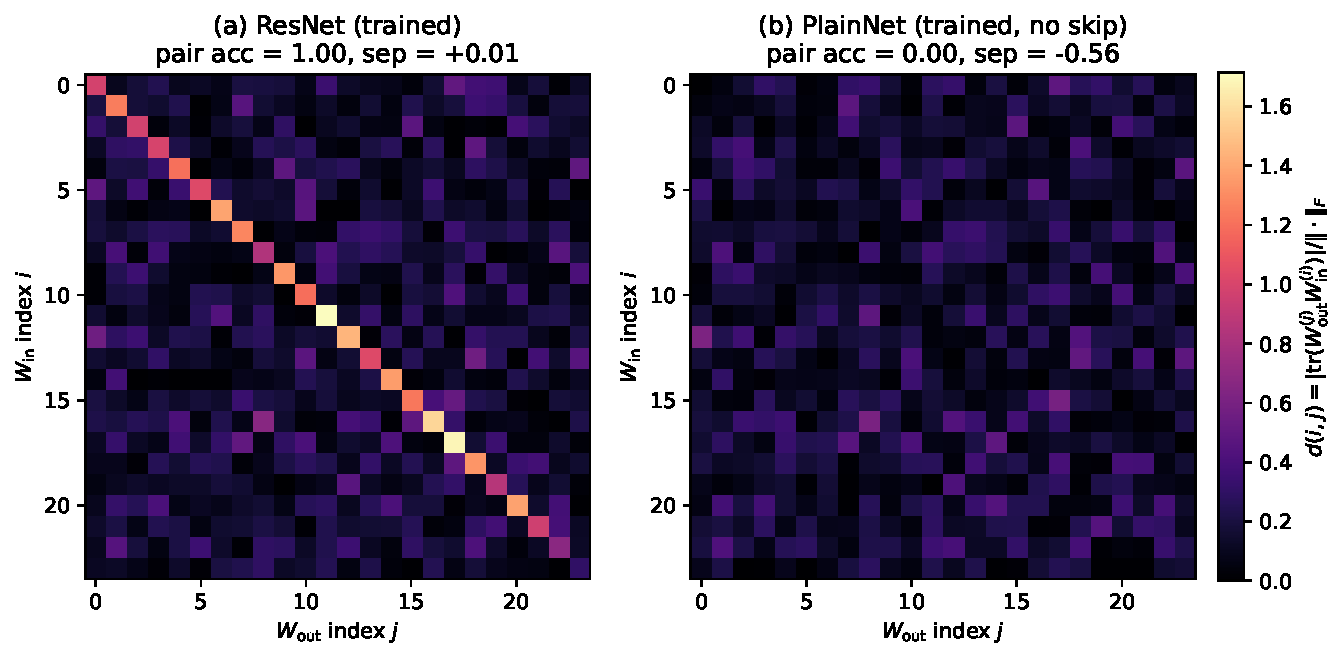
\includegraphics[width=0.85\textwidth]{../figures/fig_nonresidual_baseline.pdf}
\caption{Non-residual control experiment. \textbf{(a)} Trained ResNet: clear diagonal structure, 100\% pair accuracy. \textbf{(b)} Trained PlainNet (no skip connections): uniform noise, 0\% pair accuracy (3\% averaged over seeds). Both networks achieve comparable eval loss, confirming PlainNet learns the task but lacks the structural fingerprint.}
\label{fig:nonresidual}
\end{figure}

\paragraph{Key finding.}
The diagonal-dominance signal is not an architectural artifact but a \emph{consequence of gradient descent on residual networks}. The condition $W_{\mathrm{out}}W_{\mathrm{in}} \approx -\varepsilon I + E$ emerges early in training, sharpens monotonically, persists across architectures from residual MLPs to transformers, and \emph{requires} residual connections---non-residual networks trained on the same task show no signal.

\section{Limitations and Scope}\label{sec:limitations}

We explicitly delineate what the diagonal-dominance fingerprint does and does not establish, to preempt misreadings of the empirical results.

\paragraph{Block-level identifiability, not run-level provenance.}
The fingerprint identifies \emph{which weight matrices belong to the same residual block within a model}: given a shuffled pile of layers from one network, it recovers their original ordering. It does \emph{not} on its own distinguish two independently trained networks of the same architecture (say, two ResNet-50s with different random seeds). The trained values of $W_{\mathrm{out}}W_{\mathrm{in}}$ differ between runs in numerical detail, but both runs satisfy $W_{\mathrm{out}}W_{\mathrm{in}} \approx -\varepsilon I + E$, so both yield strong diagonal dominance and successful within-model pairing. Run-level uniqueness---using the matrix $E$ as a per-model signature---is a complementary direction we leave open. In the verification scenarios we target (e.g., confirming a deployed model matches a registered checkpoint by exact weight comparison), block-level recovery from corrupted or unlabeled weights is the relevant primitive.

\paragraph{Architecture knowledge requirement.}
The pairing procedure assumes the verifier knows (i) the architecture family (ResNet vs.\ Transformer vs.\ ConvNeXt), (ii) the residual-branch factorization to score (the $W_2W_1$ vs.\ $W_3W_2W_1$ distinction is essential for ResNet recovery; see Section~\ref{sec:experiments}, RQ1), and (iii) the layer dimensions used to reshape attention heads. This information is published with virtually every released model. When the architecture is partially unknown, the search space of factorizations is small (a few dozen candidates across the families in this paper); since the full procedure runs in seconds, exhaustive search over plausible factorizations is feasible. Recovery of pairings under \emph{adversarially obfuscated} architecture is not addressed.

\paragraph{Adversarial removal under structured transforms.}
Our 21-attack robustness sweep (Section~\ref{sec:experiments}, RQ4) covers fine-tuning at three learning rates for up to 50 epochs, alternative-target fine-tuning, and Gaussian weight noise from 1\% to 20\% relative magnitude. We have not exhaustively tested \emph{structured} attacks that preserve network function while attempting to mask the trace pattern: per-block orthogonal rotations $R \in O(h)$ applied to the hidden state ($W_{\mathrm{in}} \mapsto R W_{\mathrm{in}}$, $W_{\mathrm{out}} \mapsto W_{\mathrm{out}} R^\top$), hidden-unit permutations applied jointly to in/out projections, or learned residual additions tuned to redistribute diagonal mass. By construction, the first two are symmetries of the residual block and leave $W_{\mathrm{out}}W_{\mathrm{in}}$ \emph{invariant}---they cannot alter the diagonal-dominance score. Independent application breaks function, which contradicts the adversary's goal of preserving the deployed model. A learned residual addition tuned to break diagonal dominance is the most plausible remaining attack vector and we have not yet quantified its required perturbation magnitude. The robustness results suggest that any function-preserving perturbation large enough to destroy the fingerprint also degrades classification accuracy, but a formal lower bound on the adversarial budget is open.

\paragraph{Architectural scope.}
The method applies to architectures with identifiable residual-branch structure: residual MLPs, ResNets (full, Bottleneck, and Pre-Activation), modern ConvNets (ConvNeXt), and Transformers (both MLP and attention sublayers, encoder-only and decoder-only, full MHA and grouped-query). Plain feedforward networks without skip connections do not develop the fingerprint---as confirmed by our non-residual control experiment (Section~\ref{sec:experiments}, RQ5, Figure~\ref{fig:nonresidual}), trained PlainNets achieve only chance-level pair accuracy despite learning the task. Recurrent networks and architectures whose channel-mixing happens through non-linear gating without a linear branch product similarly fall outside the current scope. Extending the framework to non-residual architectures---potentially by identifying analogous trace conditions on Jacobian factorizations---is a natural direction, though the non-residual control suggests this would require fundamentally different structural signatures.

\section{Conclusion}\label{sec:conclusion}

We have shown that training induces an intrinsic fingerprint in neural network weights: the diagonal-dominance structure of residual-branch weight products. This signature emerges from gradient descent enforcing dynamical isometry and thus applies retroactively to any already-deployed model, enabling practical applications such as intellectual property protection and model ownership verification without requiring modifications during training.

Our empirical evaluation demonstrates the method's reliability and scope. Diagonal-dominance Hungarian matching achieves 100\% pairing accuracy on GPT-2 models from 124M to 1.5B parameters, ViT-B/16, ConvNeXt-T, and across transformer families---encoder-only BERT-base and SwiGLU+GQA Mistral-7B---with signal strength scaling as $O(\sqrt{d})$ consistent with our theoretical analysis. On ImageNet ResNets with BatchNorm, architecture-aware factorization recovers 91--100\% of correct pairs, with accuracy correlating to the number of residual blocks per stage---deeper stages yield stronger signal. The fingerprint remains robust across 21 attack configurations, degrading only when perturbations exceed approximately 20\% relative magnitude, at which point model accuracy itself collapses. Section~\ref{sec:limitations} delineates the boundaries: the fingerprint establishes block-level identity within a model rather than run-level provenance, assumes the verifier knows the architecture, and has not yet been stress-tested against function-preserving structured attacks.

Future work could extend the theoretical framework to non-residual architectures, develop cryptographic protocols that leverage these fingerprints for zero-knowledge ownership proofs, quantify adversarial budgets required to mask the trace pattern, and investigate whether similar emergent signatures arise from other optimizer families or normalization schemes.

%\acks{Acknowledgements should go at the end, before appendices and references. You can uncomment this for the camera-ready version on paper acceptance.}

\bibliography{acml26}

\end{document}
